\documentclass[journal,letterpaper]{IEEEtran}

\usepackage{cite}
\usepackage{graphicx}
\usepackage{amsmath,amssymb}
\usepackage{algorithm}
\usepackage{algorithmic}
\usepackage{psfrag}

\IEEEoverridecommandlockouts

% Better references, I think
\renewcommand{\sec}[1]{Section~\ref{sec:#1}}
\newcommand{\fig}[1]{Figure~\ref{fig:#1}}
\newcommand{\alg}[1]{Algorithm~\ref{alg:#1}}

% Algorithmic changes
\renewcommand{\algorithmicforall}{\textbf{for each}}

%% PSO Stuff
\DeclareMathOperator*{\argmin}{arg\;min}
\DeclareMathOperator*{\argmax}{arg\;max}
\DeclareMathOperator*{\arginf}{arg\;inf}
\DeclareMathOperator*{\argsup}{arg\;sup}
\providecommand{\pers}{\ensuremath{P}}
\providecommand{\neigh}{\ensuremath{N}}
\providecommand{\leftind}{\ensuremath{L}}
\providecommand{\rightind}{\ensuremath{R}}
\providecommand{\nURand}{\ensuremath{U^\neigh}}
\providecommand{\pURand}{\ensuremath{U^\pers}}
\providecommand{\ppos}{\ensuremath{\Vec{x}}}
\providecommand{\fppos}{\ensuremath{\Vec{fx}}}
\providecommand{\pvel}{\ensuremath{\Vec{v}}}
\providecommand{\nbest}{\ensuremath{\Vec{x}^\neigh}}
\providecommand{\fnbest}{\ensuremath{\Vec{fx}^\neigh}}
\providecommand{\pbest}{\ensuremath{\Vec{x}^\pers}}
\providecommand{\fpbest}{\ensuremath{\Vec{fx}^\pers}}
\providecommand{\constriction}{\ensuremath{\chi}}
\providecommand{\ncoeff}{\ensuremath{\phi^\neigh}}
\providecommand{\pcoeff}{\ensuremath{\phi^\pers}}
\providecommand{\obs}{\ensuremath{\Vec{\xi}}}
\providecommand{\ofunc}{\ensuremath{f}}
\providecommand{\swarm}{\ensuremath{swarm}}

%SpecExPSO Stuff
\providecommand{\indic}{\ensuremath{I}}
\providecommand{\specvel}{\ensuremath{\vec{V}}}
\providecommand{\specpos}{\ensuremath{\vec{X}}}
\providecommand{\leftn}{\ensuremath{\Vec{x}^\leftind}}
\providecommand{\rightn}{\ensuremath{\Vec{x}^\rightind}}
\providecommand{\caseset}{\ensuremath{\mathcal{C}}}
\providecommand{\casegen}{\ensuremath{c}}
\providecommand{\casedef}{\ensuremath{(\pbest,\nbest)}}
\providecommand{\casexn}{\ensuremath{(S,-)}}
\providecommand{\casexx}{\ensuremath{(S,S)}}
\providecommand{\casexl}{\ensuremath{(S,\leftind)}}
\providecommand{\casexr}{\ensuremath{(S,\rightind)}}
\providecommand{\casepn}{\ensuremath{(-,-)}}
\providecommand{\casepl}{\ensuremath{(-,\leftind)}}
\providecommand{\casepr}{\ensuremath{(-,\rightind)}}
\providecommand{\casepN}{\ensuremath{(-,N)}}
\providecommand{\casexN}{\ensuremath{(S,N)}}
\providecommand{\noeval}[1]{\ensuremath{#1^{-e}}}
\providecommand{\nonbest}[1]{\ensuremath{#1^{-n}}}
\providecommand{\p}{\ensuremath{p}}
\providecommand{\pset}{\ensuremath{\mathbf{p}}}
\providecommand{\s}{\ensuremath{s}}
\providecommand{\sset}{\ensuremath{\mathbf{s}}}
\providecommand{\nsset}{\ensuremath{\mathbf{ns}}}
\providecommand{\n}{\ensuremath{n}}
\providecommand{\nset}{\ensuremath{\mathbf{n}}}
\providecommand{\nnset}{\ensuremath{\mathbf{nn}}}

%Other math
\providecommand{\prob}{\ensuremath{\mathrm{Pr}}}

\title{\ \\ \LARGE\bf Speculative Evaluation in Particle Swarm Optimization%
\thanks{Matthew Gardner, Andrew McNabb, and Kevin Seppi are with the Department
of Computer Science, Brigham Young University, 3361 TMCB, Provo, UT 84602
(phone: 801-422-8717; email: \{mjg82,a,k\}@cs.byu.edu).}%
}

\date{}

\author{Matthew Gardner, Andrew McNabb, and Kevin Seppi}

\begin{document}
\maketitle

\begin{abstract}

Particle swarm optimization (PSO) has previously been parallelized primarily by
distributing the computation corresponding to particles across multiple
processors.  In these approaches, additional processors can only add more
particles to the swarm.  However, in many cases this is not efficient when
scaled to very large swarm sizes (on very large clusters).  In this paper we
present a different way of using additional processors in the computation of
PSO motivated by speculative execution in modern computer hardware.  We call
our method Speculative Evaluation in PSO (SEPSO).

In SEPSO future positions of the particles are speculated and evaluated in
parallel with the evaluation of current positions.  We show that a set of
speculative evaluation threads can be constructed such that the set will always
include the position and corresponding evaluation that would normally have
occurred at the next iteration of standard PSO.  Thus SEPSO performs two
iterations of PSO at once, allowing it to achieve better fitness faster.  Not
only can SEPSO can achieve better fitness in the same number of iterations, it
also reaches better fitness for the same number of total function evaluations
in large scale parallel environments.

Speculative Evaluation in PSO can be enhanced by diverging from the behavior of
the standard PSO to make better use of the information obtained by the
speculative evaluations.  Using these algorithmic modifications, we see
dramatic improvements in the effectiveness of the algorithm. 

\end{abstract}

\section{Introduction}
\label{sec:intro}

Particle swarm optimization (PSO) has been found to be a highly robust and
effective algorithm for solving many types of optimization problems.  For much
of the algorithm's history, PSO was run serially on a single machine.  However,
the world's computing power is increasingly coming from large clusters of
processors.  In order to efficiently utilize these resources for
computationally intensive problems, PSO needs to run in parallel.

Within the last few years, researchers have begun to recognize the need to
develop parallel implementations of PSO, publishing many papers on the subject.
The methods they have used include various synchronous algorithms
\cite{mcnabb-2007-parallel-pso-using-mapreduce,belal-2004-parallel-models-for-pso,chu-2006-intelligent-parallel-pso,jin-2005-pso-antenna-designs,parsopoulos-2004-parallel-vector-evaluated-pso,schutte-2004-parallel-global-optimization-with-pso}
and asynchronous algorithms
\cite{koh-2006-parallel-asynchronous-pso,mostaghim-2006-multi-objective-pso-on-grids,venter-2005-parallel-pso-asynchronous-evaluations}.  Parallelizing the
evaluation of the objective function can also be done in some cases, though
that is not an adaption of the PSO algorithm itself and thus is not the focus
of this paper.

These previous parallel techniques distribute the computation needed by the
particles in the swarm over the available processors.  If more processors are
available, these techniques increase the number of particles in the swarm,
either by adding individual particles or by adding entire new sub-swarms, but
in all cases the number of processors never exceeds the number of particles.
The number of iterations of PSO that the algorithms can perform is thus
inherently limited by the time it takes to evaluate the objective
function---additional processors add more particles, but do not make the
iterations go any faster.

For many functions there comes a point of diminishing returns with respect to
adding particles.  In \fig{evals-sphere} we show the value obtained after
20,000 function evaluations (not iterations) as a function of swarm size for
the well-know benchmark function Sphere (20 dimensions, reporting the average
of thirty runs).  Increasing the swarm size from 10 to 50 has a significant
effect on the value obtained.  However, increasing the swarm size from 100 to
200 makes the algorithm less efficient, that is, it reduces the progress the
algorithm makes per evaluation.  For this reason, previous work has recommended
the use of a swarm size of 50 for this function~\cite{bratton-2007-defining-a-standard-for-pso}.  Thus, in
at least some cases, adding particles indefinitely will not yield an efficient
implementation. 

\begin{figure}
  \centering
  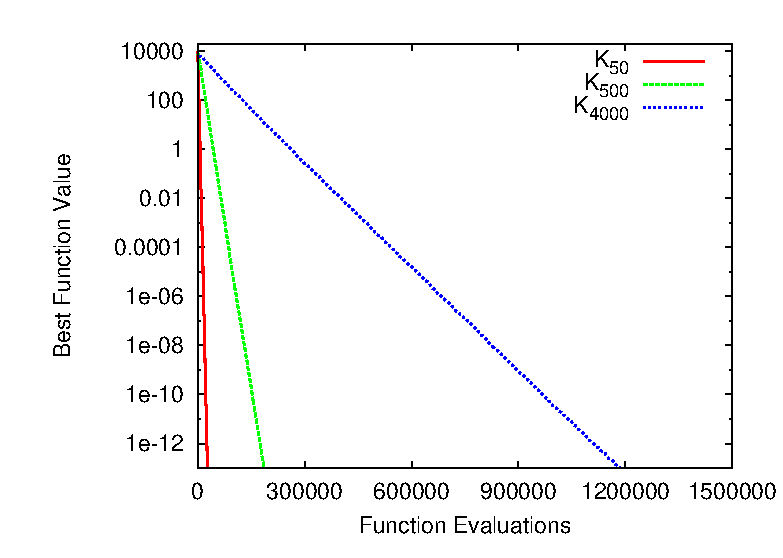
\includegraphics[width=.8\columnwidth]{evals_sphere}
  \caption{Function Sphere with a swarm with various swarm sizes.}
  \label{fig:evals-sphere}
\end{figure}

In this paper we consider PSO parallelization strategies for clusters of
thousands of processors and functions for which a single evaluation will take
at least tens of seconds, but probably minutes or perhaps hours.  Our purpose
is to explore the question of what to do with a thousand processors when 50 or
100 particles is the recommended swarm size, and simply increasing the swarm
size encounters diminishing returns.

To solve this problem, we propose a method for performing two iterations of PSO
at the same time in parallel that we call speculative evaluation.  The name
comes from an analogy to speculative execution (also known as branch
prediction) techniques commonly used in processors.  Modern processors, when
faced with a branch on which they must wait (e.g. a memory cache miss), guess
which way the branch will go and start executing, being careful not to make
changes that cannot be undone.  If the processor guesses right, execution is
much farther ahead than if it had just idly waited on the memory reference.  If
it guesses wrong, execution restarts where it would have been anyway.  

%\begin{quote}
%SKIP SKIP
%
%No really, try reading without this! The idea of speculative execution can be applied to some types of optimization
%algorithms.  When the next sampling position of the algorithm does not depend
%on the value of the objective function at the current position,
%future positions can be speculated and evaluated in parallel with the current
%position.
%This is trivially true for optimization by random sampling, for example.
%The next random sample does not depend on the previous point nor on the value
%of the objective function at that point in any way.
%It depends only on a random number.
%There is no need to wait to see
%what objective function value was obtained at the previous point,
%evaluation of the object function at the next point can begin as soon as the next random number is drawn.
%In other optimization algorithms, the next position depends on the previous position, but not the
%value obtained there, a random walk for example.
%In this case
%the next position to be evaluated
%depends only on the previous position and a random number.
%In this case, as it was in the case of random sampling,
%the object function evaluation of the next position can be done in parallel
%because it 
%does not depend on the \emph{value} of the objective function at the previous position.
%There are an infinite number of possible next positions, but only one given the draw of the random number.
%
%In still other cases, the next position to be evaluated may depend on the current position and some
%discrete valued (binary, for example) test on the value obtained at the current position.
%For example, consider a greedy random walk, in which the state only advances if a better
%position is found.
%That is, if the current value is better than the previous value,
%use the sum of the current position and the random number as the next position.
%Otherwise, computer the next position using the sum of the previous position and the random number.
%In this case the objective function can be evaluated at three positions:
%(1) the value of the objective function at the current position,
%(2) the value at the position if the test turns out to be true and (3) the value at the position
%if the test turns out to be false; all in parallel.
%In this example it is important to note that we do not need the value of the objective function at the current
%point to to reduce the infinite number of possible next positions to just two alternatives.
%Choosing between these two alternatives can be done post-hoc, after the objective function value
%at the current position and at the two alternative are computed.
%For all but the most computationally-trivial objective functions, this approach saves almost half of the
%``wall-clock'' time.
%This approach has been applied to simulated annealing~\cite{witte-1991-parallel-simulated-annealing-speculative} which like the greedy random walk,
%depends on positions and a binary test.
%
%This approach can not be used in gradient methods where the
%step size for sampling typically depends on the gradient and therefor the position and 
%a set of infinitely many possible \emph{values} outcomes
%obtained at the current position (not binary or even finite).
%\end{quote}

% Use this later?
% Skip this??
% 
% Speculative evaluation is possible in PSO because the motion of particles
% depends only on the \emph{positions} of the particle and its best neighbor, not
% the \emph{value} of the objective function at those positions.  We do not have
% to wait for a particle's function evaluation to complete in order to know where
% it might move to next, so we can compute the set of all possible next positions
% and send them to be evaluated along with the particle's current position.  Once
% the current position of each particle has been evaluated, we can determine
% which of the speculatively evaluated positions matches the branch taken by the
% particle.  We have thus evaluated two iterations at once.  This can easily get
% unwieldy if the set of next possible positions for each particle is large, but
% a wise choice of topology limits that set to a reasonable size.
% 
% But the following does need some intro

In this paper we show that the results of standard PSO can be reproduced
\emph{exactly}, two iterations at a time, using a speculative approach adapted
from speculative execution. We prove that the standard PSO equation can be
factored such that a set of speculative positions can be found which will
\emph{always} include the position computed in the next iteration.  By
computing the value of the objective function for each of the speculative
positions at the same time the algorithm evaluates the objective function for
the current position, it is possible to know the objective function values for
both the current and the next iteration at the same time.  We demonstrate this
principle by implementation and show that it produces exactly the same results
as standard PSO, but two iterations at a time.  The resulting implementation
runs efficiently on large clusters where the number of processors is much
larger than a typical or reasonable number of particles, producing better
results in less ``wall-clock'' time and, surprisingly, with fewer total
function evaluations.

Furthermore, we show that if we relax the requirements of the algorithm, no
longer demanding that it strictly reproduce the exact behavior of standard PSO,
we can introduce new speculative techniques that often out-perform PSO.  These
variants make better use of the information obtained from the extra exploration
made by the speculative function evaluations.  We also explore the idea that,
like branch prediction in processors, we need not speculatively evaluate
\emph{all} possible future positions, we can accelerate the algorithm even if
we are just \emph{likely} to have guessed right.  By pruning the speculation to
just paths that are statistically likely to reproduce the paths that are
equivalent to PSO we can increase the swarm size without increasing the number
of speculative evaluations.  We also consider several recovery strategies for
cases where the pruned set of speculative evaluations does not contain the
evaluation that standard PSO would have done.  A further improvement we explore
is speculating several iterations ahead instead of just one, which is made
possible by pruning the number of speculative evaluations.

The balance of this paper is organized as follows: \sec{pso} describes the
particle swarm optimization algorithm.  \sec{sepso} describes how speculative
evaluation can be done in parallel PSO to perform two iterations at once, then
presents a comparison of the speculative algorithm with the original PSO.  In
\sec{relax}, we discuss various methods of improving the performance of
speculative evaluation in PSO, all of which break the requirement of strictly
reproducing the behavior of the original algorithm.  In \sec{conclusion} and
\sec{future} we conclude and discuss future work.

\section{Particle Swarm Optimization}
\label{sec:pso}

Particle swarm optimization was proposed in 1995 by James Kennedy and Russell
Eberhart~\cite{kennedy-1995-particle-swarm-optimization}.  The algorithm is used to intelligently search
a multi-dimensional space by mimicking the swarming and flocking behavior of
birds and other animals. It is a social algorithm that depends on interaction
between particles to quickly and consistently approximate the optimal solution
to a given objective function.

The motion of particles through the search space has three components: an
inertial component that gives particles momentum as they move, a cognitive
component where particles remember the best solution they have found and are
attracted back to that place, and a social component by which particles are
attracted to the best solution that any of their neighbors have found.

At each iteration of the algorithm, the position $\ppos_t$ and velocity
$\pvel_t$ of each particle are updated as follows:
\begin{align}
\nonumber
	\pvel_{t+1} &=
		\constriction \bigl[ \pvel_t
			+ \pcoeff\pURand_{t}\otimes(\pbest_{t} - \ppos_{t}) \\
\label{eq:velupdate}
			& \quad \quad \quad \, + \ncoeff\nURand_{t}\otimes(\nbest_{t} - \ppos_{t})
		\bigr] \\
\label{eq:posupdate}
	\ppos_{t+1} &= \ppos_{t} + \pvel_{t+1}
\end{align}
where \( \pURand_{t} \) and \( \nURand_{t} \) are vectors of independent random
numbers drawn from a standard uniform distribution, the \( \otimes \) operator
is an element-wise vector multiplication, $\pbest$ (called personal best) is
the best position the current particle has seen, and $\nbest$ (called
neighborhood best) is the best position the neighbors of the current particle
have seen~\cite{bratton-2007-defining-a-standard-for-pso}.  \( \ncoeff \), \( \pcoeff \), and \(
\constriction \) are parameters with prescribed values required to ensure
convergence (2.05, 2.05, and .73, respectively)~\cite{clerc-2002-constricted-pso}. 

There are many ways of defining the neighbors of a particle.  Changing the
neighborhood topology has a significant effect on the performance of the
algorithm and this effect varies widely by function type.  The two most common
topologies used in the literature are the Ring topology and the Complete
topology~\cite{bratton-2007-defining-a-standard-for-pso}.  In the Ring topology, each particle has one
neighbor to either side of it; in the Complete topology, every particle is a
neighbor to every other particle.  In all topologies a particle is also a
neighbor to itself in that its own position and value are considered when
updating the particle's neighborhood best, $\nbest$.  Thus with $p$ particles,
using the Ring topology each particle with index $i$ has three neighbors:
$i-1$, $i$ (itself), and $i+1$.  With the Complete topology, each particle has
$p$ neighbors.

In this paper we use these topologies as well as a parallel adaptation of the
Complete topology, called Random, that has been shown to approximate the
behavior of Complete with far less communication~\cite{mcnabb-2009-large-particle-swarms}.  In the
Random topology, each particle randomly picks two other particles to share
information with at each iteration, along with itself.  Thus in both the Ring
and the Random topologies, all particles have three neighbors.

\section{Speculative Evaluation in PSO}
\label{sec:sepso}

The PSO algorithm can be trivially parallelized by distributing the processing
needed for each particle on across processors.  But as we have seen in the
introduction, for some functions, and for large numbers of processors, just
adding particles reaches a point of diminishing returns.  That is, adding
processors does not help us reach any given level of fitness appreciably
faster.

To address this issue we present here a different use of additional processors.
Instead of adding particles we employ a speculative evaluation approach that
allows us to perform iterations two at a time.

To do so we must first refactor PSO such that the determination of the social
and cognitive components, $\nbest$ and $\pbest$, which depend upon the value of
the objective function, is separate from the rest of the computation.  For
simplicity in this explanation, we restrict our discussion here to the case of
a Ring topology with two neighbors which we will call the ``right neighbor''
and ``left neighbor,'' whose positions are represented as $\rightn$ and
$\leftn$ respectively.  Though we will only describe the case of the Ring
topology, our methods can easily be extended to arbitrary topologies.

Our refactoring hinges on the idea that there is a finite set of possible
updates to $\nbest$ and $\pbest$ at each iteration.  For the Ring topology we
are discussing there are 7 possible update cases, identified in
Table~\ref{tab:evals}.  We label each case with an identifier referring to the
source of the update; a hyphen represents no update, $L$ represents an update
to $\nbest$ coming from the left neighbor, $R$ represents an update to $\nbest$
coming from the right neighbor, and $S$ represents an update to either $\pbest$
or $\nbest$ coming from the particle itself.  As an example, $\casexn$ refers
to the case that the particle finds a new personal best, but neither it nor its
neighbors found a position that updated its neighborhood best.  In the
equations that follow, we refer to an unspecified update case as $\casegen$,
and to the set of cases collectively as $\caseset$

\begin{table}
  \caption{All possible updates for a particle with two neighbors}
  \label{tab:evals}
  \centering
  \begin{tabular}{lcc}
	Identifier&Source of $\pbest$ update&Source of $\nbest$ update\\
	\hline
	\hline
	$\casepn$&No update&No update\\
	\hline
	$\casepl$&No update&Left Neighbor\\
	\hline
	$\casepr$&No update&Right Neighbor\\
	\hline
	$\casexn$&Self&No update\\
	\hline
	$\casexl$&Self&Left Neighbor\\
	\hline
	$\casexr$&Self&Right Neighbor\\
	\hline
	$\casexx$&Self&Self\\
	\hline
  \end{tabular}
\end{table}

Next, note that the computation of $\pbest$ and $\nbest$ (and hence which case
in $\caseset$ actually occurs) is not seen in the update
equations~\eqref{eq:velupdate} and \eqref{eq:posupdate}.  This update is
usually implemented as a pair of independent if-statements, but that is a bit
awkward for our purposes.  We will instead make this mathematically explicit by
introducing a set of indicator functions, each representing a case from
Table~\ref{tab:evals}.  We can then sum over all of the cases, and the
indicator function will make all of the terms drop to zero except for the case
that actually occurs.

In what follows we will examine the indicator function and the position and
velocity update equations for a specific case, $\casexn$, as presenting
equations for every case would be tedious.  The extension to cases not
presented is straightforward.  When we are performing function minimization, we
can define the indicator function representing the case $\casexn$ by:

\begin{align}
  \nonumber
	\indic_{t+1}^{\casexn} & (\ofunc ( \ppos_{t} ) ,\ofunc(\leftn_{t}),
	\ofunc(\rightn_{t}) ,\ofunc(\pbest_{t-1}) ,\ofunc(\nbest_{t-1}))= \\
  \label{eq:deficasexn}
	&\begin{cases}
	   1 & \text{if} \ \ofunc(\ppos_{t}) < \ofunc(\pbest_{t-1}) \\
	   &\quad \wedge \quad \ofunc(\nbest_{t-1}) < \ofunc(\ppos_{t}) \\
	   &\quad \wedge \quad \ofunc(\nbest_{t-1}) < \ofunc(\leftn_{t}) \\
	   &\quad \wedge \quad \ofunc(\nbest_{t-1}) < \ofunc(\rightn_{t}) \\
	   0 & \text{otherwise}
	\end{cases}
\end{align}

For compactness in our equations we represent this without the parameters since
they can be inferred from the subscripts on $\indic_{t+1}^{\casexn}$.

We now provide notation for the velocity update equation.  Once again we use
$\casexn$ as an example:

\begin{align}
\nonumber
	\specvel_{t+1}^{\casexn} & (\pvel_t, \ppos_{t}, \leftn_{t}, \rightn_{t},
	\pbest_{t-1}, \nbest_{t-1}, \pURand_{t}, \nURand_{t}) \\
\nonumber
		&= \constriction \bigl[ \pvel_{t} +
			\pcoeff\pURand_{t}\otimes(\pbest_{t} - \ppos_{t}) \\
\nonumber
		& \quad \quad \quad \; + \ncoeff\nURand_{t}\otimes(\nbest_{t} -
		\ppos_{t}) \bigr] \\
\nonumber
		&= \constriction \bigl[ \pvel_{t} +
			\pcoeff\pURand_{t}\otimes(\ppos_{t} - \ppos_{t}) \\
\label{eq:defvcasexn}
			& \quad \quad \quad \; + \ncoeff\nURand_{t}\otimes(\nbest_{t-1} -
			\ppos_{t}) \bigr]
\end{align}

Note that we have substituted the actual values obtained for $\pbest$ and
$\nbest$ into Equation~\eqref{eq:defvcasexn}.  Since we have restricted
ourselves to a specific case, we know the values of $\pbest$ and $\nbest$ and
do not need those terms as parameters to $\specvel_{t+1}^{\casexn}$.  In this
case, $\pbest_{t}=\ppos_{t}$, as \pbest was updated by the particle's current
position, and $\nbest_{t}=\nbest_{t-1}$, as \nbest was not updated at iteration
$t$.  Again we will drop the parameters to $\specvel_{t+1}^{\casexn}$ for
compactness.

In the same way we can create notation for the position update
equation~\eqref{eq:velupdate}:
\begin{align}
\label{eq:defpcasexn}
	\specpos_{t+1}^{\casexn} & (\ppos_{t}, \pvel_{t}, \leftn_{t},
	\rightn_{t} ,\pbest_{t-1} ,\nbest_{t-1}, \pURand_{t}, \nURand_{t}) \\
\nonumber
	& = \ppos_{t} + \specvel_{t+1}^{\casexn}
\end{align}

With this notation we can re-write the original PSO velocity
equation~\eqref{eq:velupdate}, introducing our sum over cases with the
indicator functions.  The equation becomes:
\begin{align}
\nonumber
	\pvel_{t+1} &=
		\constriction \bigl[ \pvel_t
			+ \pcoeff\pURand_{t}\otimes(\pbest_{t} - \ppos_{t}) \\
\nonumber
			& \quad \quad \quad \, + \ncoeff\nURand_{t}\otimes(\nbest_{t} -
			\ppos_{t}) \bigr] \\
\nonumber
	&= \sum_{c \in \caseset} \indic_{t+1}^{c} \ \constriction \bigl[ \pvel_t
			+ \pcoeff\pURand_{t}\otimes(\pbest_{t} - \ppos_{t}) \\
\nonumber
			& \quad \quad \quad \, + \ncoeff\nURand_{t}\otimes(\nbest_{t} -
			\ppos_{t}) \bigr]  \\
\label{eq:vel2update}
	&= \sum_{c \in \caseset} \ \indic_{t+1}^{c} \ \specvel_{t+1}^{c} 
\end{align}

We can similarly re-write the position update equation~\eqref{eq:posupdate} as:
\begin{align}
\nonumber
	\ppos_{t+1} &= \ppos_{t} + \pvel_{t+1} \\
\label{eq:pos2update}
	&= \sum_{c \in \caseset} \ \indic_{t+1}^{c} \ \specpos_{t+1}^{c} 
\end{align}

The value of the objective function at $\ppos_{t+1}$ is given by:
\begin{align}
\label{eq:val2update}
	\ofunc (\ppos_{t+1}) = \sum_{c \in \caseset} \ \indic_{t+1}^{c}
	\ \ofunc(\specpos_{t+1}^{c})
\end{align}

Returning our attention to the computation of $\ppos_{t+1}$ in
\eqref{eq:pos2update} and writing it with the parameters which were omitted
above, we obtain:
\begin{align}
\nonumber
  \ppos_{t+1} &= \sum_{c \in \caseset} \\
\nonumber
	& \indic_{t+1}^{c}(\ofunc ( \ppos_{t} ) ,\ofunc(\leftn_{t}),
	\ofunc(\rightn_{t}) ,\ofunc(\pbest_{t-1}) ,\ofunc(\nbest_{t-1})) \\
\label{eq:val2updatelong}
	& \specpos_{t+1}^{c}(\ppos_{t},\pvel_{t},\leftn_{t},\rightn_{t},
	\pbest_{t-1},\nbest_{t-1},\pURand_{t}, \nURand_{t})
\end{align}

In this form the important point to notice is that there are only 7 values (for
this Ring topology) in the set formed by $\specpos_{t+1}^{c} \ c \in\ \caseset$
and that none of them depend upon $f(\ppos_t)$ or any other objective function
evaluation at iteration $t$ (note also that while there are random numbers in
the equation, they are assumed fixed once drawn for any particular particle at
a specific iteration).  Thus PSO has been refactored such that the algorithm
can begin computing all 7 of the objective function evaluations potentially
needed in iteration $t+1$ \emph{before} $f(\ppos_t)$ is computed.  Once the
evaluation of $f(\ppos_{t})$ is completed for all particles only one of the
indicator functions $\indic_{t+1}^{c}$ will be set to 1.  We will refer to
the indicator function which is set to 1 as the ``behavior preserving
indicator'' or $bp$, since it indicates which of the computations
$\ofunc(\specpos_{t+1}^{c})$ preserves the behavior of PSO.  The rest of the
computations $\ofunc(\specpos_{t+1}^{c}) \ c \in \caseset-\{bp\}$ will be
ignored, and might just as well never have been computed.  We call these
evaluations of $\ofunc(\specpos_{t+1}^{c})$ ``speculative children'' because
they may or may not be needed.

This refactoring comes at significant expense; instead of just computing
$\ofunc(\ppos_{t})$ and then $\ofunc(\ppos_{t+1})$ in the usual way, this
refactored PSO computes $\ofunc(\ppos_{t})$ and all of the
$\ofunc(\specpos_{t+1}^{c})$, eight function evaluations in this case.  The
potential value of these speculative children lies in the fact that we can
perform the computation needed for both iteration $t$ and iteration $t+1$ at
the same time.  Remember that our intent is to accelerate parallel PSO and that
we are interested in objective functions that have at least non-trivial
computational complexity.  That is, we assume that computing
$\ofunc(\ppos_{t})$ is the computationally difficult part of one iteration of
PSO.

The value of the refactoring can best be seen in a small example.  Suppose that
unlimited processors were available and that the evaluation of the objective
function took one hour. Suppose also that for each particle the computations
$\ofunc(\ppos_{t})$ and all of the $\ofunc(\specpos_{t+1}^{c})$ were sent to
separate processors and completed in parallel.  Once the values of
$\ofunc(\ppos_{t})$ have been computed for all particles, the computation
needed to determine the values of the indicator functions $\indic_{t+1}^{c}$
and to complete iteration $t+1$ is inconsequential.  In this environment all of
the function evaluations needed for two iterations of PSO could be completed in
just one hour where as the conventional implementation would require two hours
for those same two iterations.

However, we do not have an infinite number of processors at our disposal, and
performing speculative evaluation significantly increases the number of
function evaluations needed in PSO.  We show in the rest of this paper that in
many, though not all, instances the extra performance achieved by being able to
do more iterations at a time outweighs the benefit that would have been gained
by merely increasing the number of particles in the swarm.

The number of speculative evaluations needed per particle depends on the number
of neighbors each particle has.  The number of update cases in a topology where
each particle has $n$ neighbors is $2(n+1)$; there are two possibilities for
updates to $\pbest$ (updated by the particle itself and not updated), and $n+1$
possibilities for updates to $\nbest$ (updated by each neighboring particle and
not updated).  When the particle is also a neighbor to itself, as is always the
case in commonly used topologies, one of the cases can be eliminated, as a
particle cannot be the source of an update to its neighborhood best while not
also updating its personal best.  Thus we have $2(n+1)-1$, or $2n+1$,
speculative evaluations per particle.  In a swarm with $p$ particles and $n$
neighbors per particle, $(2n+1)p$ speculative evaluations are needed.

Because the number of speculative evaluations depends on the number of
neighbors a particle has, the choice of topology is an important one.  The use
of the Complete topology, where every particle is a neighbor to every other
particle, would require $O(p^2)$ speculative evaluations per iteration.
Clearly it is much more desirable to have a sparse topology, where $O(np)$ is
much smaller than $O(p^2)$.  However, some functions are better optimized with
the Complete topology and the quick spread of information it entails than with
sparse topologies.  Accordingly, we use the Random topology described
in~\cite{mcnabb-2009-large-particle-swarms}, which has been shown to effectively simulate the
Complete topology.  In~\sec{results} we report the results for performing
speculative evaluation using both the Ring topology and the Random topology on
a number of common benchmark functions.

It is not trivial in some parallel architectures to determine which speculative
position was the correct next position of each particle.  In the rest of this
section we move from the mathematics of our method to its implementation.
First we discuss the relatively easy case of a centralized parallel PSO
algorithm with a master computer and many slaves.  In such an architecture, the
master keeps track of all necessary information with only trivial message
passing needed.  Then we discuss the more complicated case of a distributed
algorithm, where each particle is on its own and needs to send and receive
messages to and from other particles.  Finally we discuss the further
complications of a dynamic topology, where a particle's neighbors change from
one iteration to another.

\subsection{Terminology}

To aid in describing our methodology, we introduce a few terms.  A particle's
set of \emph{speculative children} is the set of all possible next iteration
states that a particle could have.  We use $\p_t$ to denote a particle at
iteration $t$ and $\s_{t+1}$ to denote one of $\p_t$'s speculative children,
corresponding to one of the rows in Table~\ref{tab:evals}.  $\n_t$ is a
neighbor of particle $\p_t$.  Sets of particles are given by $\pset$, $\sset$,
or $\nset$, whereas single particles are simply $\p$, $\s$, or $\n$.

We separate each iteration of PSO into several steps.  First there is the
motion step, where a particle updates its position and velocity.  Then a
particle's position is evaluated, and the particle updates its current value
and its personal best.  Finally, a particle gets information from its neighbors
and updates its neighborhood best.

A particle at iteration $t-1$ that has been moved to iteration $t$ using
Equations~\eqref{eq:velupdate}~and~\eqref{eq:posupdate}, but whose position has
not yet been evaluated, is denoted as $\noeval{\p}_t$.  Once its position has
been evaluated, but it has still not yet received information from its
neighbors, it is denoted as $\nonbest{\p}_t$.  Only when the particle has
updated its neighborhood best is it a complete particle at iteration $t$.  It
is then simply denoted as $\p_t$.

\subsection{Centralized Algorithms}

In a centralized, or Master-Slave, parallel PSO algorithm, one machine, the
master, keeps track of all necessary information, and all other machines are
merely used to evaluate the objective function at various positions as directed
by the master~\cite{belal-2004-parallel-models-for-pso}.  To perform speculative evaluation in such
an architecture, the master generates the positions to evaluate speculatively
as in Equation~\eqref{eq:pos2update}.  After having the slaves evaluate the
objective function at all necessary positions, the master then decides which
position to accept for each particle, as in Equation~\eqref{eq:val2updatelong}.
The outline of the procedure is given in \alg{centralized}.

\begin{algorithm}
  \caption{Speculative Evaluation in a Centralized PSO}
  \label{alg:centralized}
  \begin{algorithmic}[1]
	\STATE Move all $\p_{t-1}$ to $\noeval{\p}_t$ using
	  Equations~\eqref{eq:velupdate}~and~\eqref{eq:posupdate}
	\STATE For each $\noeval{\p}_t$, get its neighbors $\noeval{\nset}_t$ and
	  generate $\noeval{\sset}_{t+1}$ according to
	  Equation~\eqref{eq:pos2update}.
	\STATE Evaluate all $\noeval{\p}_t$ and $\noeval{\sset}_{t+1}$ in parallel
	\STATE Update personal best for each $\noeval{\p}_t$ and
	  $\noeval{\s}_{t+1}$, creating $\nonbest{\p}_t$ and $\nonbest{\s}_{t+1}$
	\STATE Update neighborhood best for each $\nonbest{\p}_t$, creating
	  $\pset_t$
	\FORALL{$\p_t$}
	\STATE Pick $\nonbest{\s}_{t+1}$ from $\nonbest{\sset}_{t+1}$ that matches
	  the branch taken by $\p_t$ according to
	  Equation~\eqref{eq:val2updatelong}.
	\STATE Pass along personal and neighborhood best values obtained by $\p_t$,
	  making $\nonbest{\p}_{t+1}$
	\ENDFOR
	\STATE Update neighborhood best for each $\nonbest{\p}_{t+1}$, creating
	  $\pset_{t+1}$
	\STATE Repeat from Step 1 until finished
  \end{algorithmic}
\end{algorithm}

Given a set of particles at iteration $t-1$ (perhaps which have just been
initialized), the master must move each particle using
Equations~\eqref{eq:velupdate} and \eqref{eq:posupdate} to obtain the set
$\noeval{\pset}_t$.  For each particle $\noeval{\p}_t$, the master must get its
set of neighbors $\noeval{\nset}_t$ and use their positions, along with the
position of $\noeval{\p}_t$, to enumerate all possible combinations of $\pbest$
and $\nbest$ that particle $\noeval{\p}_t$ could end up with (as shown in
Table~\ref{tab:evals}).  Each of those combinations defines a speculative
particle, $\s_t$, that can be moved using Equation~\eqref{eq:pos2update} to
obtain $\noeval{\s}_{t+1}$.  The result is a set of particles
$\noeval{\pset}_t$, and for each particle a set of speculative children
$\noeval{\sset}_{t+1}$, which can all be evaluated at once.

The master then has the slaves evaluate the particles.  Once all particles,
speculative and original, have been evaluated and the values reported to the
master, the master determines which speculative child of each particle was the
correct one.

This is done by first updating each particle's personal and neighborhood bests.
Mathematically, this corresponds to the evaluation of an indicator function
similar to that found in Equation~\eqref{eq:deficasexn}.  In practice, this is
done by moving each $\noeval{\p}_t$ to $\nonbest{\p}_t$ and each speculative
particle $\noeval{\s}_{t+1}$ to $\nonbest{\s}_{t+1}$ by associating the value
determined by the slave to the particle it came from, and updating that
particle's personal best if the value reported is better than its previous
personal best value.  Then each $\nonbest{\p}_t$ must be updated to $\p_t$ by
updating its neighborhood best position and value with information about each
of its neighbors.  This is simply the original PSO algorithm, and corresponds
to steps 1--5 in \alg{centralized}.

Then, with the set $\pset_t$, the branch that was actually taken by each
particle can be determined, and the correct speculative child can be chosen.
The branches depend entirely on whether or not the personal best of $p_t$ was
updated and which particle, if any, updated the particle's neighborhood best.
Both of those items are now known, and the child that matches the branch is
selected as per Equation~\eqref{eq:val2updatelong} (step 7 in
\alg{centralized}).

The parent $\p_t$ must pass its personal best value to the child, as the child
knows only the position that it guessed, not the function value at that
position.  It is possible that both $\p_t$ and $\s_{t+1}$ update their personal
bests, but $\p_t$'s value is better.  For example, suppose that $\p_{t-1}$ has
a personal best value of 3, and the we are seeking to minimize the function.
$\noeval{\p}_t$ is created, and $\noeval{\s}_{t+1}$ is moved assuming that
$\p_t$ has updated its personal best with its position at time $t$.  Then both
$\noeval{\p}_t$ and $\noeval{\s}_{t+1}$ are evaluated, with values 1 and 2,
respectively.  $\nonbest{\s}_{t+1}$ would think that its current position is
its personal best, as the value it found, 2, is better than its previous
personal best value of 3.  It needs to receive the personal best value from its
parent to know that its personal best position $\pbest$ is actually the
position of $\p_t$, not $\s_{t+1}$.

The parent also needs to pass the value of the neighborhood best that the child
guessed.  The child only knows the position and needs the value in order to
make future comparisons between neighborhood best positions (step 8).

Upon picking the correct branch for each particle and updating the child's
personal best and neighborhood best value (from iteration $t$), the result is
the set $\nonbest{\pset}_{t+1}$, as the particles are now no longer
speculative.  What remains is to update the neighborhood best of those
particles from their neighbors (from iteration $t+1$), as above, to obtain
$\pset_{t+1}$.  That set of particles can subsequently be used to produce the
sets $\noeval{\pset}_{t+2}$ and $\noeval{\sset}_{t+3}$ (steps 1 and 2 in
\alg{centralized}), and the process repeats itself.

\subsection{Distributed Algorithms}

\label{sec:distributed}

In a distributed parallel PSO algorithm, individual processors not only perform
evaluations of particles, but also their movement.  The information for each
particle is not held by a central machine that directs the algorithm; instead,
each processor has the information for the particle or particles that it is in
charge of and must perform the steps of the algorithm for those particles.
Messages such as values and positions for the neighborhood best are sent
between processors.  There may still be some machine that collects information
from all of the particles and outputs the result of the algorithm, though that
machine's importance is much less than in centralized algorithms.

To perform speculative evaluation in a distributed PSO algorithm, there must be
some way to have processors evaluate the speculative children of particles,
without giving the speculative particles the same treatment as actual
particles, as the speculative children only live for one iteration.  One way
that can be done is by assigning each particle a set of machines instead of a
single machine, and the particle directs its extra machines to evaluate its
speculative children.  However the distributed framework functions, the same
information needs to be passed between particles, and we describe here the
messages each particle needs to receive to perform speculative evaluation.

A processor that is controlling a single particle $\p_{t-1}$ must first move
the particle to $\noeval{\p}_t$ and produce the particle's speculative children
$\noeval{\sset}_{t+1}$.  This is done in the same way as described above.
However, in order to produce $\noeval{\sset}_{t+1}$, the processor needs
information about the particle's neighbors, so there must be some message
passing to get that information.  Particularly, the information that the
processor needs is the position of each of the particle's neighbors at
iteration $t$.

To get that information, a round of message passing is required.  Each particle
sends its position to its neighbors at iteration $t$, so that all particles can
generate $\noeval{\sset}_{t+1}$.  After each particle evaluates its position
and the positions of its speculative children, it passes information about the
outcome of iteration $t$ to its neighbors, so that neighboring particles can
update their neighborhood bests to move from $\nonbest{\p}_t$ to $\p_t$.  Once
that communication is finished, the particle can select the speculative child
which matched the branch that iteration $t$ actually produced.  Then another
round of information passing follows, for iteration $t+1$, so that
$\nonbest{\p}_{t+1}$ can be updated to $\p_{t+1}$.  Two iterations have then
been completed with only one round of evaluations, and the next iteration can
start again with the first round of message passing.

In some distributed frameworks, like the MapReduce framework that we used in
our experiments, rounds of message passing can be expensive.  The method just
described uses three rounds of message passing for every two iterations
(corresponding to steps 2, 5 and 10 in \alg{centralized}).  It is possible to
perform speculative evaluation in PSO with only one round of communication per
two iterations.  However, the methodology is tedious and is not the focus of
this paper, so we defer its description to the Appendix.

\subsection{Dynamic Topologies}

Performing speculative evaluation in PSO with a dynamic topology raises a
sticky issue of its own.  In a static topology, at iteration $t$ a particle
already has all of the information about the positions of its neighbors during
iterations $1$ through $t-1$.  If the neighbor finds a better position at
iteration $t$, the particle updates its neighborhood best, but if it does not,
it still has its old neighborhood best from its neighbors for all previous
iterations.

In a dynamic topology, a particle might not have information about the previous
positions of its neighbors at iteration $t$.  That means that its new
neighborhood best could come not only from its neighbors' positions at
iteration $t$, but also from their personal best from iteration $t-1$, as
neighbors' personal bests are what are used to update a particle's neighborhood
best.  That creates a problem for speculative evaluation---there are
potentially more than $2n+1$ possible next positions, increasing the amount of
work that must be done to perform the second iteration at the same time as the
first.

This is easily fixed by updating each new particle $\noeval{\p}_{t+2}$ with the
currently available information about its neighbors $\noeval{\nset}_{t+2}$
before producing its children $\noeval{\sset}_{t+3}$.  If a particle
$\noeval{\p}_{t+2}$ updates its neighborhood best with the personal bests of
$\noeval{\nset}_{t+2}$ before calculating the next possible positions for
$\noeval{\sset}_{t+3}$, there are still only $2n+1$ possible next positions,
and the problem is avoided.

\subsection{Comparison with Standard PSO}
\label{sec:results}

We ran experiments to compare our speculative PSO algorithm to the standard PSO
algorithm.  At each iteration of the algorithms, we use one processor to
perform one function evaluation for one particle, be it speculative or
non-speculative.  We acknowledge that for benchmark functions with very fast
evaluations this may not be the best use of parallelism in PSO.  But for many
real-world applications, the objective function takes on the order of minutes
or more to evaluate; in such cases our choice of framework is reasonable.

The speculative algorithm actually performs two iterations of PSO at each
``iteration,'' so we instead call each ``iteration'' a round of evaluations.

To use the same number of processors (and hence evaluations) for each
algorithm, speculative evaluation must use a smaller swarm size than standard
PSO.  For each of the topologies we used, a particle has three neighbors
including itself.  As shown in Table~\ref{tab:evals}, this results in $7$
speculative evaluations per particle.  With one evaluation needed for the
original, non-speculative particle, we have $8p_s$ evaluations for every two
iterations, where $p_s$ is the number of particles in the speculative swarm.
The extra evaluations done in speculative evaluation would instead be particles
in regular PSO, so we compare swarms of size $p_s$ in speculative evaluation
with swarms of size $8p_s$ in regular PSO.

Where the Complete topology would normally be used, we use a Random topology in
our speculative algorithm, as Complete leads to an explosion in the number of
speculative evaluations.  If speculative evaluation were not being performed,
it is possible that the Complete topology would be used.  However, the Complete
topology also requires a very large amount of interprocessor communication in
parallel PSO, so it is still quite possible that Random would be used even with
standard PSO.  But, to be fair in our comparisons, we compare to the standard
PSO algorithm using both the Random topology with two neighbors and the
Complete topology.  All functions have 20 dimensions, and all results shown are
averages over 20 runs.  We use 240 processors in our experiments (except where
otherwise noted), so our speculative algorithm uses 30 particles and standard
PSO uses 240 particles.  For ease of labeling, we call our speculative
algorithm SEPSO and standard PSO just PSO, with the topology following.

First we look at the function Sphere, the simplest of common benchmark
functions.  Its equation is $f(\Vec{x}) = \sum_{i=1}^D x_i^2$.  The function
has no local optima and is best optimized in terms of function evaluations with
a small swarm using a Complete topology.  Accordingly, we show results for a
Complete swarm in \fig{basic-sphere}.  We can see that when both SEPSO and PSO
are using a Random topology, SEPSO clearly outperforms PSO.  However, the
comparison between SEPSO and PSO Complete is not as encouraging---PSO Complete
performs slightly better.

\begin{figure}
  \centering
  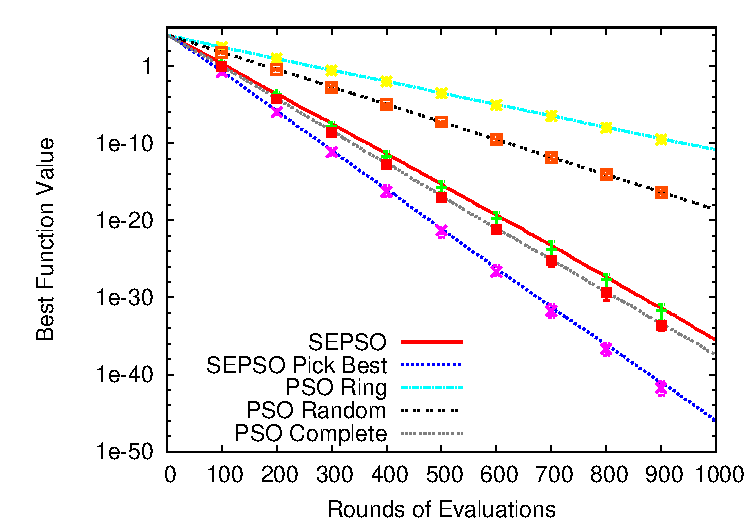
\includegraphics[width=.8\columnwidth]{sphere}
  \caption{Function Sphere with a swarm that uses 240 processors per round of
  evaluations.  Our speculative algorithm has a swarm of 30 particles and does
  two iterations per round, while standard PSO algorithms use 240 processors
  and do one iteration per round.}
  \label{fig:basic-sphere}
\end{figure}

Next we look at the function Griewank, defined by the equation $f(\Vec{x}) =
\frac{1}{4000} \sum_{i=1}^D x_i^2 - \Pi_{i=1}^D \cos\left(\frac{x_i}{\sqrt{i}}
\right) + 1$.  It is generally recommended to use the Ring topology when
optimizing the Griewank function, as Complete is prone to premature convergence
on a local optimum.  Griewank has a global optimum with a value of 0, and
sometimes the swarm finds the optimum and sometimes it doesn't.  Instead of
showing average function value at each iteration, a more accurate plot for
Griewank shows the percent of runs that have found the global optimum by each
iteration.  We show results in \fig{basic-griewank2} for swarms of size 30 and
240 using the Ring topology.  One can see in the figure that the SEPSO
algorithm finds the optimum faster than the original PSO.  However, because the
swarm size is so small, SEPSO gets stuck a little less than half of the time.

\begin{figure}
  \centering
  \includegraphics[width=.8\columnwidth]{griewank2}
  \caption{Function Griewank with a swarm that uses 240 processors per round of
  evaluations.  Instead of showing average function value, we show the
  percentage of runs that have found the global optimum by each iteration.}
  \label{fig:basic-griewank2}
\end{figure}

Because our speculative algorithm got stuck with such a small swarm size, we
ran a set of experiments on Griewank with 800 processors, giving swarms of size
100 and 800 instead of 30 and 240.  \fig{basic-griewank3} shows the results.
\fig{basic-griewank3} is very similar to \fig{basic-griewank2}, except that
speculative evaluation finds the global optimum essentially 100\% of the time.
Thus with a few more processors, our algorithm finds the optimum twice as fast
as the original PSO without a significant loss of accuracy.

\begin{figure}
  \centering
  \includegraphics[width=.8\columnwidth]{griewank3}
  \caption{Function Griewank with a swarm that uses 800 processors per round of
  evaluations.}
  \label{fig:basic-griewank3}
\end{figure}

Lastly we look at a function that does not show any kind of improvement with
this method.  The function Rastrigin is defined as $f(\Vec{x}) = \sum_{i=1}^D
\left(x_i^2 - 10\cos\left(2\pi x_i\right) + 10\right)$.  It has been shown that
with Rastrigin, the more particles there are in the swarm, the lower function
value it finds, up to at least 4000 particles~\cite{mcnabb-2009-large-particle-swarms}.  Smaller
swarms get caught in local optima.  Because our speculative algorithm has a
significantly smaller swarm size, it gets stuck at higher values while the
larger swarms performing regular PSO continue to improve the best value found.
\fig{rastrigin} shows the results graphically.

\begin{figure}
  \centering
  \includegraphics[width=.8\columnwidth]{rastrigin}
  \caption{Function Rastrigin with a swarm that uses 240 processors per round
  of evaluations.}
  \label{fig:rastrigin}
\end{figure}

\section{Relaxing the Requirements}
\label{sec:relax}

While the idea of speculative evaluation in particle swarm optimization is
intriguing, the results of the previous section show that in many cases it
requires too many extra evaluations to produce competitive results.  On most
functions, the larger swarm size that can be used in regular PSO leads to
better performance than is found by trying to do speculative evaluation.
However, if we keep the idea of speculative evaluation while relaxing the
requirement of exactly reproducing the behavior of the original PSO algorithm,
we see some impressive results.

We outline three main improvements to speculative evaluation.  First, in
\sec{pickbest} we describe a method that uses all of the information found in
doing speculative evaluations.  Then Sections~\ref{sec:pruning}
through~\ref{sec:wrong} present a technique that reduces the number of
speculative evaluations that need to be done for each particle.  Finally,
\sec{manyiters} shows a method for speculating several iterations ahead,
instead of just one.  

\subsection{Pick the Best Child}
\label{sec:pickbest}

In performing speculative evaluation as we have described it, $2n+1$
speculative evaluations are done per particle, while all but one of them are
completely ignored.  We can try to make use of those evaluations instead of
throwing them away.  

To use the extra speculative evaluations, instead of choosing the speculative
child that matches the branch that the original PSO would have taken (the
``behavior preserving'' branch), we take the child that has the best value.
The methodology is exactly the same as above except for the process of choosing
which speculative child to accept.  The only change needed in \alg{centralized}
is in step 7, where the $\noeval{\s}_{t+1}$ with the best value is chosen from
$\noeval{\sset}_{t+1}$ instead of with the matching branch.

This can be thought of as drawing a number of samples from the next iteration
and accepting the best one.  Speculative particles that move in good directions
are kept.  It seems this modification to PSO would produce more exploitation,
decreasing the amount of exploration.  With functions that are less deceptive
we would expect this method to work well, while performance on more deceptive
functions would probably be hurt.

We show in \fig{sphere-pickbest} the results of using this modification on the
function Sphere.  For ease of labeling, we call the modified algorithm Pick
Best.  As can be seen, where SEPSO did not manage to perform as well as PSO
Complete, Pick Best handily outperforms it with the same number of processors.

\begin{figure}
  \centering
  \includegraphics[width=.8\columnwidth]{sphere2}
  \caption{Function Sphere with a swarm that uses 240 processors per round of
  evaluations, comparing Pick Best with previous results.}
  \label{fig:sphere-pickbest}
\end{figure}

Sphere is a function for which very little exploration needs to be done, so
always keeping the best speculative position found makes intuitive sense.  A
less intuitive result occurs when using Pick Best with the function Griewank.
Griewank is a highly deceptive function prone to premature convergence.  Our
intuition on the behavior of picking the best speculative child is that it
would tend to prematurely converge more often than the original PSO.  However,
as seen in \fig{griewank-pickbest}, Pick Best increases the chance of finding
the optimum while also reducing the number of iterations required to converge.
Perhaps Pick Best encourages local exploitation, while the sparse communication
of the Ring topology still allows for global exploration.

\begin{figure}
  \centering
  \includegraphics[width=.8\columnwidth]{griewank4}
  \caption{Function Sphere with a swarm that uses 240 processors per round of
  evaluations, comparing Pick Best with previous results.}
  \label{fig:griewank-pickbest}
\end{figure}

\subsection{Pruning the Speculative Evaluations}
\label{sec:pruning}

Because the problem facing speculative evaluation is having too many possible
evaluations to perform, a natural step to take is to eliminate some of the
evaluations.  If we could reliably predict which branch were going to be taken,
we could limit ourselves to one speculative evaluation per particle instead of
$2n+1$.  As not all of the branches are evaluated in any given iteration, we
call this technique pruning.  

A naive approach to pruning is to keep track of the last branch taken by each
particle and speculate on that branch.  This turns out to be correct far less
than half of the time on average.

A more principled approach would be to use the statistical behavior of PSO to
find probabilities of taking any particular branch.  While we cannot with
certainty predict which branch a particle will take every time, if we can use
statistics to narrow down the $2(n+1)$ possible evaluations to a few likely
candidates, we can decrease the amount of computation required to do
speculative evaluation and improve our performance.

\subsection{Branch Statistics}

In Table~\ref{tab:evals} we presented all possible branches that a particle
with two neighbors could take.  Here we lump all of the neighbors together and
consider the statistics for the five branches shown in
Table~\ref{tab:branches}.  In the identifiers, N represents an update to
$\nbest$ coming from any neighbor.

\begin{table}[ht]
  \caption{Five Branches to Consider for Statistics}
  \label{tab:branches}
  \centering
  \begin{tabular}{lcc}
	Identifier&Source of $\pbest$ update&Source of $\nbest$ update\\
	\hline
	\hline
	$\casepn$&No update&No update\\
	\hline
	$\casexn$&Self&No update\\
	\hline
	$\casexx$&Self&Self\\
	\hline
	$\casepl$&No update&Some Neighbor\\
	\hline
	$\casexl$&Self&Some Neighbor\\
	\hline
  \end{tabular}
\end{table}

\begin{table}[ht]
  \caption{Branch Statistics in PSO}
  \label{tab:stats}
  \centering
  \scriptsize
  \begin{tabular}{c|c|c|c|c|c|c}
	Topology&Function&\casepn&\casexn&\casexx&\casepN&\casexN\\
	\hline
	\hline
	Ring&Sphere&53.0\%&9.3\%&11.4\%&20.2\%&6.2\%\\
	&Griewank&51.7\%&8.4\%&12.2\%&20.7\%&7.0\%\\
	&Rastrigin&49.5\%&4.8\%&14.6\%&21.3\%&9.9\%\\
	&Rosenbrock&51.3\%&7.4\%&12.9\%&21.1\%&7.3\%\\
	\cline{2-7}
	&Average&{51.3\%}&{7.5\%}&{12.8\%}&{20.8\%}&
	{7.6\%}\\
	\hline
	\hline
	Random&Sphere&66.7\%&11.9\%&2.6\%&15.6\%&3.1\%\\
	&Griewank&69.0\%&10.9\%&2.5\%&14.9\%&2.7\%\\
	&Rastrigin&81.9\%&5.5\%&1.5\%&10.0\%&1.0\%\\
	&Rosenbrock&74.2\%&7.7\%&2.2\%&14.0\%&1.8\%\\
	\cline{2-7}
	&Average&{73.0\%}&{9.0\%}&{2.2\%}&{13.6\%}&
	{2.2\%}\\
	\hline
	\hline
	Complete&Sphere&31.9\%&9.2\%&0.2\%&45.1\%&13.5\%\\
	&Griewank&35.3\%&8.4\%&0.2\%&44.1\%&11.9\%\\
	&Rastrigin&47.7\%&6.7\%&0.2\%&38.2\%&7.0\%\\
	&Rosenbrock&35.3\%&3.4\%&0.3\%&54.4\%&6.6\%\\
	\cline{2-7}
	&Average&{37.6\%}&{6.9\%}&{0.2\%}&{45.5\%}&
	{9.8\%}\\
	\hline
  \end{tabular}
\end{table}

Row 1 in Table~\ref{tab:branches}, \casepn, corresponds to the phenomenon
commonly called stagnation in the literature, but only with a single particle.
As an interesting aside, we found that complete stagnation (where the entire
swarm is stagnant) practically never occurs in PSO, though frequently large
percentages of the swarm are stagnant.  Iterations where the entire swarm is
stagnant average less than 2 in 1000 iterations, unless the swarm converges
beyond machine precision.  When graphs of the best function value flat-line,
what really has happened is a contraction of the particles' velocity, not
stagnation in the technical sense.  

We seek to find the probability of taking any given branch, given whatever
information is needed: $\prob(\caseset_t|\cdot)$.  In finding these
probabilities, we do not attempt to derive any distribution from the PSO
equations, we simply look at empirical distributions.  However, even with
empirical distributions, the problem with this approach is that it is not clear
what information influences the probability of taking a branch.  The failure of
the naive approach seems to say that the previous branch, $\caseset_{t-1}$, is
not incredibly useful.  We look at two factors that we believe have a
significant influence on $\prob(\caseset_t)$: topology and function.  Thus we
are looking at $\prob(\caseset_t|T,F)$.

We show in Table~\ref{tab:stats} with what percentage a particle takes each of
these branches for three different topologies and four different functions.
All of our statistics are from swarms of 240 particles.  Brief experimentation
showed that other swarm sizes had similar statistics.  We ran 750 iterations on
all combinations of functions and topologies except for the functions Griewank
and Rastrigin with the Complete topology.  We found that those runs frequently
converged past machine precision after 500 iterations, and that led to
erroneously high values for the probability of stagnation.  Instead we ran for
only 450 iterations on those two combinations.  All of our results were
averaged over 20 runs of the algorithm; thus the probabilities presented are
the averages of 3.6 million trials for the branch taken (2.16 million for the
two with only 450 iterations).  Table~\ref{tab:stats} contains the results.  We
have already defined the functions Sphere, Griewank, and Rastrigin.  Rosenbrock
is defined as $f(\Vec{x}) = \sum_{i=1}^D
\left(100(x_{i+1}-x_i^2)+(x_i-1)^2\right)$.

The probabilities presented in Table~\ref{tab:stats} are interesting in and of
themselves and could probably be used to better understand the characteristics
of various topologies.  It is notable that there is small variation between
functions in any given topology, but the variation across topologies is far
greater.  However, our concern is with speculative evaluation.  We are
interested in predicting the branch that any given particle will take at a
particular iteration.  For our purposes, it appears that given a topology, the
probability of selecting a branch and the function are close to independent, or
$\prob(\caseset_t|T,F) \approx \prob(\caseset_t|T)$.

From Table~\ref{tab:stats} we can see that with the Random topology, we can
pick the first branch, corresponding to stagnation, and be right around 70\% of
the time.  With the Ring topology, we would be right 50\% of the time.
Branches \casepN and \casexN really correspond to several actual branches, as
all of the neighbors are lumped together.  The 20\% probability of taking
branch \casepN with the Ring topology can be split into two branches, as there
are only two neighbors.  It also turns out that the neighbor that last updated
the neighborhood best is the most likely to update it next time, so keeping
track of that information could be fruitful in trying to predict that branch.

The statistics for the Complete topology are less promising, as there are 240
neighbors that branch \casepN splits into, instead of two.  Pruning does,
however, allow for the possibility of using the Complete topology in
speculative evaluation while avoiding the explosion in the number of
evaluations it would otherwise entail.  Though pruning makes its use possible,
we still found the communication costs in our parallel environment prohibitive,
so we do not present any results for the Complete topology here.

With the other topologies, however, there are a few branches with very high
probabilities, so we can have hope that cutting out some of the evaluations
that have low probability will lead to an increase in overall performance.  In
order to implement this kind of pruning, the only change that needs to be made
to \alg{centralized} is in Step 2, where the speculative children are
generated.  Instead of generating all possible speculative children, generate
the subset of the children that is desired.

\subsection{What if we guessed wrong?}
\label{sec:wrong}

When not all of the branches are evaluated, there is some probability of not
evaluating the branch that was actually taken by the original particle.  We 
need to decide what to do in this case.  

One possibility is to leave the particle as it is, not accepting any of the
speculative evaluations, because none of them were correct.  This leads to
particles being at different iterations, as some particles guess correctly
while others do not.  Thus we lose exact compatibility with the original PSO,
though this particular relaxation is nothing new; asynchronous adaptations of
PSO do the same thing.  As an aside, it is equivalent in this case to simply
increment the iteration number of particles which fail to correctly predict
their branch.  This keeps the iteration number constant across all particles,
simplifying the work needed to be done in determining neighbors when dynamic
topologies are involved.  We call this technique Social Promotion.

Another possibility is to pick the best child, as described in \sec{pickbest}.
This ignores the fact that the branch might have been wrong; it does not
matter, because we simply accept the child that had the best value.  In most of
the experiments that we ran, it turned out that picking the best child
performed better than keeping the particle back an iteration.

There are a large number of ways to prune speculative evaluations.  We
experimented with several, but present results only for one possible pruning.
The pruning we present uses only the two most probable branches in the Random
topology.  As seen in Table~\ref{tab:stats}, these are the two branches where
the $\nbest$ value was not updated---\casepn and \casexn.  Those branches are
also convenient in that no messages are needed from neighbors in order to
produce the positions of the speculative particles---in distributed frameworks
using several rounds of communication (see \sec{distributed}), one of the
rounds of communication can be dropped entirely.

Because we are now only doing two speculative evaluations per particle (along
with evaluating the original particle), with 240 processors we can have a swarm
of size 80, instead of the 30 particles in previous experiments.  

In \fig{sphere-pruned}, we show the results of this simple pruning on the
function Sphere.  As can be seen, the larger number of particles that pruning
allows results in better results when picking the best speculative child.  
When rejecting all speculative children no real improvement is seen over the
original PSO algorithm.

\begin{figure}
  \centering
  \includegraphics[width=.8\columnwidth]{sphere3}
  \caption{Function Sphere with a swarm that uses 240 processors per round of
  evaluations, comparing pruning with previous results.}
  \label{fig:sphere-pruned}
\end{figure}

When looking at the function Griewank, presented in \fig{griewank-pruned}, we
see different results.  Our intuition about picking the best child is more
correct in this case; while adding 50 more particles to the swarm, Pick Best
with pruning still gets stuck more often than the original Pick Best.  However,
Social Promotion does well in this case, finding the optimum every time and
faster than the original PSO.

\begin{figure}
  \centering
  \includegraphics[width=.8\columnwidth]{griewank5}
  \caption{Function Griewank with a swarm that uses 240 processors per round of
  evaluations, comparing pruning with previous results.}
  \label{fig:griewank-pruned}
\end{figure}

\subsection{More than one iteration ahead}
\label{sec:manyiters}

We need not simply produce speculative children for the next iteration.  We can
view all possible speculative evaluations for a particle as an infinite tree
with branching factor $2n+1$.  As we have already seen that doing one full
level of the tree produces too many extra evaluations to be profitable, it is
incredibly unlikely that doing two full iterations would produce decent
results.  But, if the idea of speculating more than one iteration ahead is
combined with wisely pruning the possible evaluations based on branch
statistics, we can use just a few extra evaluations to go two or more
iterations ahead on the most likely branches.

When speculating more than one iteration ahead, the idea of Social Promotion
cannot feasibly be implemented, as we can only determine correct branches for
the first iteration.  Thus in this case we always pick the child that has the
highest value.

The question of which branches to take in this infinite tree is an intriguing
one that we can only begin to explore here.  If the branch corresponding to
stagnation has a 75\% chance of being taken, as in the Random topology with
most functions, we could speculate three iterations ahead on that branch and
still have a 42\% chance of predicting correctly.  However, intuition would say
that perhaps it is better to hope that the particle is productive instead of
stagnant, so a branch where the particle updates its personal best might be
more fruitful to try.  In our experiments we try just one of the countless
possibilities, but that one turns out to work very well.  More work is needed
to compare the different branching possibilities on various functions.

The combination of branches we tried uses seven speculative evaluations per
particle, matching the swarm size of the original speculative algorithm.  The
seven evaluations we used corresponded to several iterations of branches
\casepn and \casexn.  Two of the evaluations were just one iteration ahead,
four were two iterations ahead, and one was three iterations ahead.  The
evaluations that were one iteration ahead were branches \casepn and \casexn;
those that went two iterations ahead were formed by taking either branch
\casepn or \casexn and then branch \casepn or \casexn; and the evaluation going
three iterations ahead followed branch \casepn on all three iterations.

The results when optimizing the function Sphere, presented in
\fig{sphere-manyiters}, are rather astounding.  When 240 processors are
available for use, performing speculative evaluation several iterations ahead
finds values an average of 46 orders of magnitude better than using the
processors to perform the standard PSO algorithm with 240 particles.

\begin{figure}
  \centering
  \includegraphics[width=.8\columnwidth]{sphere4}
  \caption{Function Sphere with a swarm that uses 240 processors per round of
  evaluations, comparing speculating several iterations ahead with previous
  results.}
  \label{fig:sphere-manyiters}
\end{figure}

With the function Griewank, the premature convergence problems inherent in
picking the best child are exacerbated when speculating several iterations
ahead.  When the algorithm finds the optimum, it finds it quicker than any
other method we tried.  However, it also gets stuck and fails to find the
optimum more than any other method.  In order for this method to be
consistently useful on functions like Griewank, it seems that more processors
are required.  The results are shown in \fig{griewank-manyiters}.

\begin{figure}
  \centering
  \includegraphics[width=.8\columnwidth]{griewank6}
  \caption{Function Griewank with a swarm that uses 240 processors per round of
  evaluations, comparing speculating several iterations ahead with previous
  results.}
  \label{fig:griewank-manyiters}
\end{figure}

\section{Conclusions}
\label{sec:conclusion}

We have described a new technique for using processors in parallel PSO to
improve the performance of the algorithm.  To our knowledge, this is the first
time extra processors have been used to do anything in PSO besides increase the
swarm size.  In an increasingly parallel world, such advancements will prove to
be crucial to the continued effectiveness of PSO.

We have detailed how to perform speculative evaluation in PSO in several
different parallel frameworks.  Using this methodology, the behavior of the
original PSO algorithm can either be exactly reproduced, two iterations at a
time, or the behavior can be modified in order to improve performance.  While
exactly reproducing PSO often uses too many extra processors to be useful, when
we allow ourselves some freedom with the algorithm we see great improvements
over previous methods.  We have shown results that conclusively demonstrate the
superiority of our techniques for several functions over naively adding
particles to the swarm when extra processors are available.

Though our methods show great improvements on some functions, they do not work
for all functions.  As is commonly known, in PSO there is a trade-off between
exploration and exploitation.  Some functions need only minimal exploration,
and some never seem to have enough.  Increasing the swarm size is a natural way
to increase exploration in a parallel environment.  However, once ``enough''
exploration has been reached for any particular function, adding additional
particles adds only incremental benefits.  A better use of the additional
processors, as we have shown, is to perform some amount of speculative
evaluation.

Sphere is a function for which only a very small amount of exploration needs to
be done, and our speculative methods show improvements on Sphere of over 40
orders of magnitude.  Such functions are perfect for our methods.

Rastrigin, on the other hand, is a function for which increasing the swarm size
up to 4000 particles still shows improvements in the performance of the
algorithm.  With such functions, the smaller swarm size required by speculative
evaluation is not able to produce enough exploration to perform better than
standard PSO at the swarm sizes we were able to experiment with.

Griewank is a function in between Sphere and Rastrigin.  It is highly deceptive
and is prone to premature convergence, but by adding particles to the swarm a
point is reached where ``enough'' exploration is done, and the algorithm finds
the optimum essentially all of the time.  For such functions, the best approach
seems to be to increase the swarm size until ``enough'' exploration is reached,
then use extra processors to perform speculative evaluation and increase the
number of iterations performed.  Sphere and Rastrigin can be thought of as
special cases of these types of functions; Sphere simply needs a very small
swarm size to produce ``enough'' exploration, and Rastrigin requires a very
large swarm.  We expect that for all functions there is a swarm size for which
additional particles are less useful than additional iterations.

Large parallel clusters are often required to successfully optimize practical
modern problems.  To properly use PSO with such clusters, a balance needs to be
made between using processors to increase the swarm size and using them to
increase the speed of the algorithm.  This work is a first step in that
direction.

\section{Future Work}
\label{sec:future}

This work represents the first attempt of which we are aware at using
additional processors in parallel with PSO to do something other than either
add particles to the swarm or parallelize the evaluation of the objective
function.  We anticipate that many future advancements can be made.

We have speculated that our Pick Best method simply draws a number of samples
from the next iteration of the sampling distribution of PSO and keeps one of
them.  It would then be expected that the sampling distribution of that method
is very similar to the distribution of the original PSO.  This remains to be
proven, or even demonstrated empirically.

We gave a passing glance to some very interesting statistical characteristics
of PSO.  Our motivation was to use the statistics to improve our speculative
algorithm, but it seems there are some nuggets in the numbers that could be
used to improve our understanding of the behavior of PSO in general, and what
role a topology plays.  A potentially very fruitful avenue of future work would
be to further analyze the branch statistics in PSO across many functions and
topologies, categorizing both the topologies and the functions and discovering
what it is that makes certain topologies work well with certain functions.
There are also some particles that seem to drive the swarm and others that are
stagnant almost the entire time.  Such information could be used in a
TRIBES-like fashion~\cite{clerc-2003-tribes} to determine which particles should be
removed from the swarm, perhaps starting them close to well-performing
particles.

We turned what used to be a very simple algorithm with only one major parameter
to tweak (the topology) into a convoluted mess with countless possibilities for
speculative evaluations.  Perhaps future research will be able to narrow down
the endless possibilities into the few best ones, making the algorithm simple
again.  We have presented some small amount of exploration of the possible
alternatives, but our discussion is by no means exhaustive or conclusive.

Our methods for determining which speculative evaluations to perform were
independent of the particle; all particles performed the same number and type
of evaluations.  Another way to allocate speculative evaluations is to somehow
use the performance of each particle to determine how many and which extra
evaluations it can have.  We imagine that the benefits of intelligently and
dynamically deciding which particles get extra evaluations could produce very
good results.  Future work could explore the use of a centralized allocator for
extra processors or ideas in the multi-robot task allocation literature, such
as auctions, to better assign processors to particles for speculative
evaluations.  While such methods involve extra communication, with long-running
function evaluations the extra overhead of intelligently allocating resources
would likely be negligible.

A technique similar to ours has been previously used to parallelize simulated
annealing~\cite{witte-1991-parallel-simulated-annealing-speculative}.  Any other optimization algorithm that only
depends on current sampling positions when computing the next position to
sample can be parallelized with this technique.  In particular, genetic
algorithms produce future generations by combining individuals from the current
generation.  With a large population size there would be an unwieldy amount of
possible future individuals, but the potential exists to modify the algorithm
to use some kind of speculative evaluation.  A related but quite distinct
technique for reducing computation in evolutionary algorithms was proposed
in~\cite{poli-2006-backward-chaining-evolutionary-algorithms}.

\appendix[Alternate form of message passing]

Here we describe a method that requires only one round of communication for
each pair of iterations, which happens at step 5 of \alg{centralized}.  Many
more messages are needed, but that is sometimes more desirable than
synchronizing all of the machines three times.

This second method only requires one round of passing information because
information about iterations $t$ and $t+1$ is passed at the same time.  Each
processor reconstructs from the messages it receives all of the information
that it needs about its neighbors.  Messages are passed directly after
evaluating each particle and its children, so all messages are of the form of
$\nonbest{\p}_t$ or $\nonbest{\s}_{t+1}$.  The first iteration needs to be
treated specially, so each particle can produce its initial set of speculative
children---neighbors need only pass their initial position.  This kind of
message passing necessitates the careful use of random seeds, so that when each
processor computes the motion equations for its neighbors it gets the same
results as its neighboring processors.

With the results of evaluating $\noeval{\p}_t$ and $\noeval{\sset}_{t+1}$,
along with all of the required messages from neighboring particles, the goal is
to produce $\p_{t+1}$ and output $\noeval{\p}_{t+2}$ and $\noeval{\sset}_{t+3}$
ready to be evaluated for the next iteration.  We first focus on the messages
needed to produce $\p_{t+1}$.

Upon evaluation, $\noeval{\p}_t$ becomes $\nonbest{\p}_t$, needing only to get
its neighborhood best information from its neighbors.  All of its neighbors,
then, must send it a message, so that from their updated personal best at
iteration $t$ the particle becomes $\p_t$.  The work done with the messages
received thus far is just as in regular PSO, and is graphically depicted in 
\fig{messages1}.

\begin{figure}
  \centering
  \psfrag{pt-n}[C][C]{$\nonbest{\p}_{t}$}
  \psfrag{nt-n}[C][C]{$\nonbest{\nset}_{t}$}
  \psfrag{pt}[C][C]{$\p_{t}$}
  \includegraphics[width=.3\columnwidth]{messages1}
  \caption{The production of $\p_{t}$ from the original particle
  $\nonbest{\p}_{t}$ and the messages $\nonbest{\nset}_{t}$.}
  \label{fig:messages1}
\end{figure}

With $\p_t$ we can select the correct speculative child as described above and
produce $\nonbest{\p}_{t+1}$.  Again we show the use of messages thus far
graphically, in \fig{messages2}.  

\begin{figure}
  \centering
  \psfrag{pt-n}[C][C]{$\nonbest{\p}_{t}$}
  \psfrag{nt-n}[C][C]{$\nonbest{\nset}_{t}$}
  \psfrag{pt}[C][C]{$\p_{t}$}
  \psfrag{pt1-n}[C][C]{$\nonbest{\p}_{t+1}$}
  \psfrag{st1-n}[C][C]{$\nonbest{\sset}_{t+1}$}
  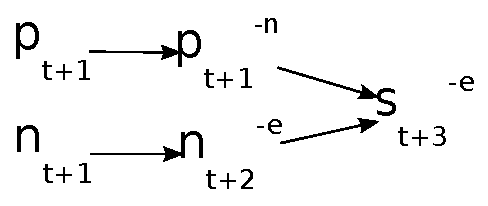
\includegraphics[width=.5\columnwidth]{messages2}
  \caption{The production of $\nonbest{\p}_{t+1}$ from the original particle 
  $\nonbest{\p}_{t}$, messages $\nonbest{\nset}_{t}$ and
  $\nonbest{\sset}_{t+1}$, and intermediate particles.}
  \label{fig:messages2}
\end{figure}

We then need the set of neighbors to $\nonbest{\p}_{t+1}$,
$\nonbest{\nset}_{t+1}$, so we can update $\nonbest{\p}_{t+1}$'s neighborhood
best.  To produce each neighbor $\nonbest{\n}_{t+1}$, we need the same
information for the neighboring particle that we needed to produce the original
particle, $\nonbest{\p}_{t+1}$; we need the original neighbor particle, its
speculative children, and its neighbors.  With that information, the set
$\nonbest{\nset}_{t+1}$ can be obtained by following the same process used to
obtain $\nonbest{\p}_{t+1}$.  We graphically show the messages needed to
produce $\nonbest{\nset}_{t+1}$ in \fig{messages3}.  Note that it looks
identical to \fig{messages2}, just with different sets of particles.

\begin{figure}
  \centering
  \psfrag{nt-n}[C][C]{$\nonbest{\nset}_{t}$}
  \psfrag{nnt-n}[C][C]{$\nonbest{\nnset}_{t}$}
  \psfrag{nt}[C][C]{$\nset_{t}$}
  \psfrag{nt1-n}[C][C]{$\nonbest{\nset}_{t+1}$}
  \psfrag{nst1-n}[C][C]{$\nonbest{\nsset}_{t+1}$}
  \includegraphics[width=.6\columnwidth]{messages3}
  \caption{The production of each $\nonbest{\n}_{t+1}$ from the original
  particle $\nonbest{\n}_{t}$, messages $\nonbest{\nnset}_{t}$ and
  $\nonbest{\nsset}_{t+1}$, and intermediate particles.  $\nnset$ is the set of
  neighbors for each particle $\n$, and $\nsset$ is the set of $\n$'s
  speculative children.  Note the similarity between this and \fig{messages2}.}
  \label{fig:messages3}
\end{figure}

With $\nonbest{\nset}_{t+1}$ and $\nonbest{\p}_{t+1}$, we can produce
$\p_{t+1}$.  This is shown in \fig{messages4}.  Note that we just combined
Figures~\ref{fig:messages2}~and~\ref{fig:messages3}, putting them together
to make $\p_{t+1}$, as all the particle needs is its neighborhood best to be
updated.

\begin{figure}
  \centering
  \psfrag{pt-n}[C][C]{$\nonbest{\p}_{t}$}
  \psfrag{nt-n}[C][C]{$\nonbest{\nset}_{t}$}
  \psfrag{pt}[C][C]{$\p_{t}$}
  \psfrag{pt1-n}[C][C]{$\nonbest{\p}_{t+1}$}
  \psfrag{st1-n}[C][C]{$\nonbest{\sset}_{t+1}$}
  \psfrag{nt-n}[C][C]{$\nonbest{\nset}_{t}$}
  \psfrag{nnt-n}[C][C]{$\nonbest{\nnset}_{t}$}
  \psfrag{nt}[C][C]{$\nset_{t}$}
  \psfrag{nt1-n}[C][C]{$\nonbest{\nset}_{t+1}$}
  \psfrag{nst1-n}[C][C]{$\nonbest{\nsset}_{t+1}$}
  \psfrag{pt1}[C][C]{$\p_{t+1}$}
  \includegraphics[width=.8\columnwidth]{messages4}
  \caption{The production of $\p_{t+1}$ from the original particle 
  $\nonbest{\p}_{t}$, messages $\nonbest{\nset}_{t}$, $\nonbest{\sset}_{t+1}$,
  $\nonbest{\nnset}_{t}$, and $\nonbest{\nsset}_{t+1}$, and intermediate
  particles.  Note that this is just a combination of \fig{messages2} and
  \fig{messages3}.}
  \label{fig:messages4}
\end{figure}

In order to get $\p_{t+1}$, then, a particle needs to receive messages from its
neighbors, its neighbors' neighbors, its speculative children, and its
neighbors' speculative children.  The particle $\p_{t+1}$ can be passed to some
central machine to track the progress of the algorithm, and it can be moved to
$\noeval{\p}_{t+2}$ in order to start the next iteration.

The next goal is to produce the set $\noeval{\sset}_{t+3}$.  As described
above, the necessary components to produce $\noeval{\sset}_{t+3}$ are
$\noeval{\p}_{t+2}$ and the neighbors of $\noeval{\p}_{t+2}$,
$\noeval{\nset}_{t+2}$.  We already have $\noeval{\p}_{t+2}$, so what remains
is to produce $\noeval{\nset}_{t+2}$.  It is sufficient to obtain
$\nset_{t+1}$, as each neighbor particle $\n_{t+1}$ can be moved with the
motion equations to $\noeval{\n}_{t+2}$.

We have already described how to use a set of messages to obtain $\p_{t+1}$.
The process is exactly the same to produce each $\n_{t+1}$, requiring the same
messages, only for the neighbor particles instead of the particle itself.
\fig{messages5} shows graphically how $\noeval{\sset}_{t+3}$ is produced.

\begin{figure}
  \centering
  \psfrag{pt1}[C][C]{$\p_{t+1}$}
  \psfrag{nt1}[C][C]{$\nset_{t+1}$}
  \psfrag{nt2-e}[C][C]{$\noeval{\nset}_{t+2}$}
  \psfrag{pt2-e}[C][C]{$\noeval{\p}_{t+2}$}
  \psfrag{st3-e}[C][C]{$\noeval{\sset}_{t+3}$}
  \includegraphics[width=.5\columnwidth]{messages5}
  \caption{The production of $\noeval{\p}_{t+2}$ and $\noeval{\sset}_{t+3}$
  from $\p_{t+1}$ and $\n_{t+1}$, each of which are produced as in
  \fig{messages4}.}
  \label{fig:messages5}
\end{figure}

Having obtained both $\noeval{\p}_{t+2}$ and $\noeval{\sset}_{t+3}$ from the
messages received, the algorithm then moves to the evaluation phase, and the
process repeats itself.  The particles are evaluated, send their messages, and
produce the next set of particles to be evaluated from the messages received.

To perform the entire process, at each message passing round a particle must
receive messages from its neighbors, its neighbors' neighbors, its neighbors'
neighbors' neighbors, its speculative children, its neighbors' speculative
children, and its neighbors' neighbors' speculative children.  With the Ring
topology, that looks like more messages than it really is, as many of the
neighbors' neighbors are duplicates.  With the Random topology, however, the
list of necessary messages could be rather large.  

One more issue arises when dealing with dynamic topologies.  With neighbors
changing each iteration, messages that processors pass to their neighbors need
to be sent to the correct neighbors for each iteration.  A particle cannot
simply send messages to its neighbors' neighbors' neighbors---it needs to send
messages to its iteration $t$ neighbors' iteration $t+1$ neighbors, and so on.
For every neighbor outward information is sent, the iteration also needs to be
incremented, as information about neighbors' neighbors is used during iteration
$t+1$, and information about neighbors' neighbors' neighbors is used to
reconstruct information about iteration $t+2$.  Also, this method of message
passing again requires the use of random seeds if the topology is random, so
that each processor computes the same neighbors for a particle as all other
processors.

This may seem like an inordinate amount of work, and with some distributed PSO
frameworks it is.  However, other parallel frameworks necessitate this type of
message passing, so we have described how speculative evaluation can be
performed in those circumstances.


\bibliographystyle{unsrt}
\bibliography{%
../../../bib/aml/bib,%
../../../bib/pso/general/bib,%
../../../bib/pso/parallel/bib,%
../../../bib/pso/topology/bib,%
../../../bib/sim-anneal/parallel/bib,%
../../../bib/ga/bib}

\end{document}
